% Activate the following line by filling in the right side. If for example the name of the root file is Main.tex, write
% "...root = Main.tex" if the chapter file is in the same directory, and "...root = ../Main.tex" if the chapter is in a subdirectory.
 
%!TEX root =  ../book_example.tex


\chapter[Short Title]{Full Title}

\section{Introduction}
\lipsum[3]
En ekvation för framtiden: 
\begin{flalign}\label{eqn:tvapol}
    I = \frac{E-U}{R_0} &&
\end{flalign}
Och en liten för dåtiden: 
\begin{flalign}\label{eqn:tvapol2}
	I_k = \frac{E}{R_0}. &&
\end{flalign}
\lipsum[1-2]
\begin{figure}[tb]
    \centering
    \begin{circuitikz}[american voltages]
        \draw (0,0) to[V=$V_{in}$] (0,3)
        to[R=$R_1$] (2,3)
        to[R=$R_2$] (2,0)
        -- (0,0);
        \draw (2,3) to[short,-*] (3,3);
        \node[right] at (3,3) {$V_{out}$};
    \end{circuitikz}
    \caption{Voltage divider circuit. OBS AI-genererad dummy bild.}
    \label{fig:voltage_divider}
\end{figure}
\begin{example}
            [tvåpolsuppmätning -- batteri]
        \label{ex:tvapolsmatning}
        \hfill \break
        Ett batteris polspänning mäts för några olika
        strömmar som ställs in med hjälp av ett variabelt
        motstånd (t.ex., en vridpotentiometer).
        Mätuppställningen visas i figuren nedan.
        Vridpotentiometern ändras så att strömmen genom
        batteriet ökar i jämna steg, varvid spänningen över
        polerna mäts vid varje ström.
        \begin{center}
            \begin{circuitikz}[american voltages]
                \draw (0,0) rectangle ++ (1,2.5) ;
                \node[rotate=90, anchor=center] at
                (0.5,1.25) {Batteri} ;
                \draw (1, 2) -- ++ (1.5 ,0)
                to[ammeter, i=$I$] ++ (2,0)
                to[vR,l=Vridpot.] ++ (0,-1.5)
                to[short,-*] ++ (-2.5,0)
                to[voltmeter,  v<=$U$, -*] ++(0, 1.5) ;
                \draw (1, 0.5) -- ++ (1, 0) ;
            \end{circuitikz}
        \end{center}
        I diagrammet nedan visar cirklarna de uppmätta
        spänningarna för respektive ström, linjen är en
        approximation av karakteristiken för att
        underlätta.
        \begin{center}
            % baserat på arnes handritade, men omvänd:
            % chap02/c02fig09/Ex.2.11_copy_tvapol.jpg
            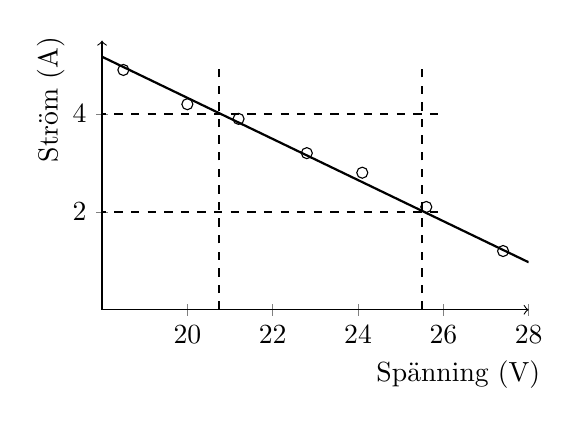
\begin{tikzpicture}
                \begin{axis}[
                    width=7cm, height=5cm,
                    axis lines=middle,
                    axis line style={->},
                    xmin=18, xmax=28,
                    ymin=0, ymax=5.5,
                    xlabel={Spänning (V)},
                    ylabel={Ström (A)},
                    xlabel style={
                        at={(axis description cs:1.05,0)},
                        anchor=north east,
                        yshift=-15pt},
                    ylabel style={
                        at={(axis description cs:0,1.05)},
                        anchor=south east,
                        rotate=90,
                        yshift=10pt},
                    domain=18:28,
                    ]

                    % Ideal linje
                    \addplot[black, thick]
                    { 4.75 - 0.42*(x - 19) } ;

                    % Streckade linjer
                    \addplot[
                    black,
                    dashed,
                    thick
                    ] coordinates {
                        (25.5,0)
                        (25.5,5)
                    };

                    \addplot[
                    black,
                    dashed,
                    thick
                    ] coordinates {
                        (20.75,0)
                        (20.75,5)
                    };

                    \addplot[
                    black,
                    dashed,
                    thick
                    ] coordinates {
                        (0,2)
                        (26,2)
                    };

                    \addplot[
                    black,
                    dashed,
                    thick
                    ] coordinates {
                        (0,4)
                        (26,4)
                    };

                    % Fejkade mätpunkter
                    \addplot[
                    only marks,
                    mark=o,
                    mark size=2pt,
                    black
                    ] coordinates {
                        (18.5,4.9)
                        (20,4.2)
                        (21.2,3.9)
                        (22.8,3.2)
                        (24.1,2.8)
                        (25.6,2.1)
                        (27.4,1.2)
                    };
                \end{axis}
            \end{tikzpicture}
        \end{center}
        Bestäm batteriets källresistans, tomgångsspänning
        och kortslutningsström.
        \HRule
        \noindent\textbf{Lösning:}\\
        En rät linje anpassas till mätpunkterna, denna syns
        som en heldragen linje i figuren ovan.
        Först beräknar vi lutningen på linjen, vi tar hjälp
        av de streckade linjerna, läser av i figuren och
        räknar lutningen,~$k$:
        \begin{flalign*}
            &k = \frac{\Delta I}{\Delta U}
            = \frac{2-4}{\num{25.5}-\num{20.5}}
            = \num{-0.4}. && \\
            \intertext{Källresistansen är negativ
                invers på lutningen:}
            &R_0 = \frac{-1}{k} = \frac{-1}{\num{-0.4}}
            = \qty{2.5}{\ohm}. &&
        \end{flalign*}
        Tomgångsspänningen, $E$, kan bestämmas genom att
        sätta in värdena för en mätpunkt längs linjen i
        ekv.~\eqref{eqn:tvapol}. Vi sätter tex. in värdena
        för den första mätpunkten, $I = \qty{4.9}{\A}$ och
        $U = \qty{18.5}{\V}$, i ekv.~\eqref{eqn:tvapol}:
        \begin{flalign*}
            \num{4.9} = \frac{E-\num{18.5}}{\num{2.5}}
            \implies E = \num{4.9} \cdot \num{2.5}
            + \num{18.5} = \qty{30.75}{\V}. &&
        \end{flalign*}
        Kortslutningsströmmen, $I_k$, kan sedan bestämmas
        med hjälp av ekv.~\eqref{eqn:tvapol2}:
        \begin{flalign*}
            I_k = \frac{E}{R_0}
            = \frac{\qty{30.75}{\V}}{\qty{2.5}{\ohm}}
            = \qty{12.3}{\A}. &&
        \end{flalign*}
\end{example}

